\documentclass[12pt]{book}
\usepackage[margin=.85in]{geometry} % for MARGIN
\usepackage[many]{tcolorbox}    	% for COLORED BOXES (tikz and xcolor included)


\usepackage{multicol}   
\usepackage{enumerate}
\usepackage[shortlabels]{enumitem}
\usepackage{varwidth}
\usepackage{tasks}
\usepackage[export]{adjustbox}

\usepackage{titleps}
\usepackage{setspace}               % for LINE SPACING
\usepackage[⟨options⟩]{fancyhdr}
\usepackage{enumitem}
\setlist{nosep}
\usepackage{tikz}
\usepackage{pgfplots}
\pgfplotsset{compat=1.5.1}
\usetikzlibrary{datavisualization}
\usetikzlibrary{datavisualization.formats.functions}

\newcommand{\D}{\displaystyle}


\setlength\parindent{0pt}   % killing indentation for all the text
\setstretch{1.3}            % setting line spacing to 1.3
\setlength\columnsep{0.25in} % setting length of column separator
\pagestyle{fancy}           % setting pagestyle to be headings

\usepackage[]{titlesec}

\fancyhead[L]{Math V04 - College Algebra}
\fancyhead[R]{Christina Papazacharioudakis}

\tcbset{
    sharp corners,
    colback = white,
    before skip = 0.2cm,    % add extra space before the box
    after skip = 0.5cm      % add extra space after the box
}                           % setting global options for tcolorbox

    \newtcolorbox{boxR}{
    fontupper = \color{black}, % font color
    boxrule = 1.5pt,
    colframe = black,
    rounded corners,
    arc = 5pt   % corners roundness
}

\definecolor{ballblue}{rgb}{0.13, 0.67, 0.8}

\begin{document}



\begin{comment}
Name: \underline{\hspace{100mm}}
\vspace{20mm}
  \centerline{\Large \textbf{Chapter 2: Equations and Inequalities} } 

{\large
\begin{center}
\begin{varwidth}{\textwidth}
\begin{enumerate}[2.1]
    \item The Regular Coordinate System and Graphs
    \item Linear Equations in One Variable
    \item Models and  Applications (Skipping)
    \item Complex Numbers
    \item Quadratic Equations
    \item Other Types of Equations
    \item Linear Inequalities and Absolute Value Inequalities
\end{enumerate}
\end{varwidth}
\end{center}

}
\newpage  
\end{comment}

{\Large \textbf{6.5 Logarithmic Properties}}

We now explore the rules (or properties) of logarithms that help us solve equations involving exponents and logarithms. Let’s begin by learning some fundamental rules when working with logarithms.

\vspace{3mm}
\textbf{{\large The Product Rule for Logarithms}}

As we have seen in the previous sections, logarithms are exponents. Let's review the product rule for exponents:


\vspace{10mm}

This property of exponents, coupled with the awareness that a logarithm is an exponent, suggests the \textbf{product rule for logarithms}:
\vspace{1mm}

\centerline{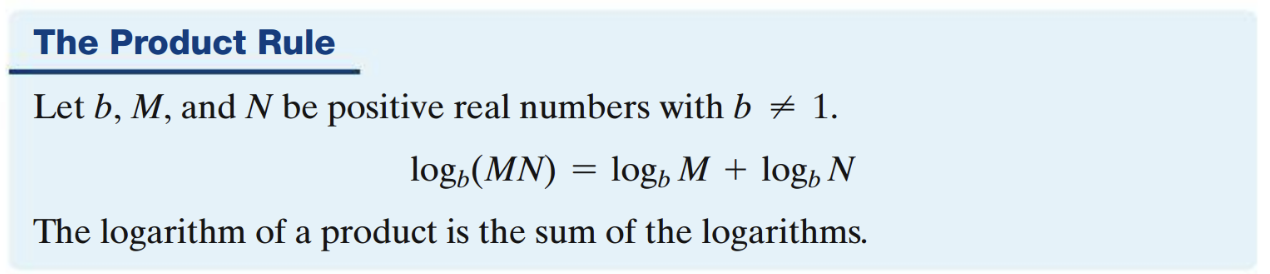
\includegraphics[scale=.7]{Chapter 6/6.6-figure1.png}}
Let's take a look at why this is true:

\vspace{50mm}

\underline{\textbf{Example 1 - Using the Product Rule for Logarithms}}

Use the product rule to expand each of the logarithmic expressions:
\begin{multicols}{3}
    \begin{enumerate}[(a)]
    \item $\D \log_4(7\cdot5)$
    \item $\D \log(10x)$
    \item $\D \log_5(x^2-36)$
\end{enumerate}
\end{multicols}

\newpage

\textbf{{\large The Quotient Rule for Logarithms}}

Let's review the quotient rule for exponents:


\vspace{20mm}

This property of exponents, coupled with the awareness that a logarithm is an exponent, suggests the \textbf{quotient rule for logarithms}:
\vspace{1mm}

\centerline{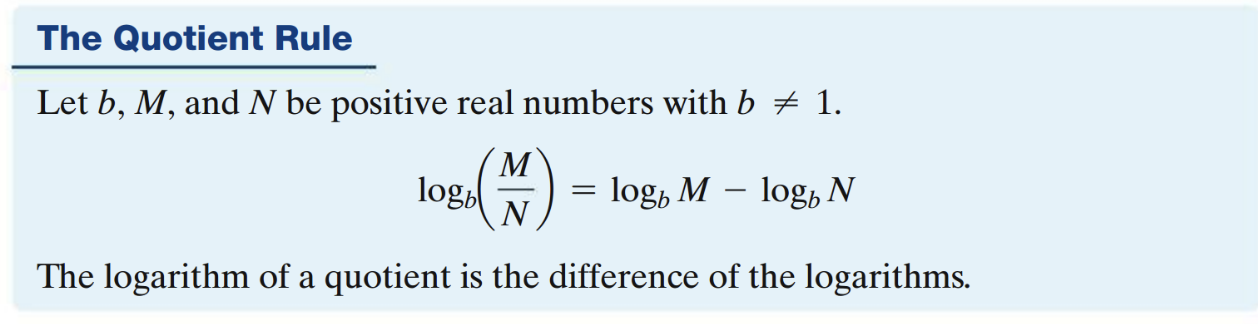
\includegraphics[scale=.7]{Chapter 6/6.6-figure2.png}}
Let's take a look at why this is true:

\vspace{50mm}

\underline{\textbf{Example 3 - Using the Quotient Rule for Logarithms}}

Use the quotient rule to expand each of the logarithmic expressions:
\begin{multicols}{3}
    \begin{enumerate}[(a)]
    \item $\D \log_7\left(\frac{19}{x}\right)$
    \item $\D \ln\left(\frac{e^3}{7}\right)$
    \item $\D \log_2\left(\frac{x}{(2-x)(3x+4)}\right)$
\end{enumerate}
\end{multicols}

\newpage


\textbf{{\large The Power Rule for Logarithms}}

Let's review the power rule for exponents:


\vspace{20mm}

This property of exponents, coupled with the awareness that a logarithm is an exponent, suggests the \textbf{power rule for logarithms}:
\vspace{1mm}

\centerline{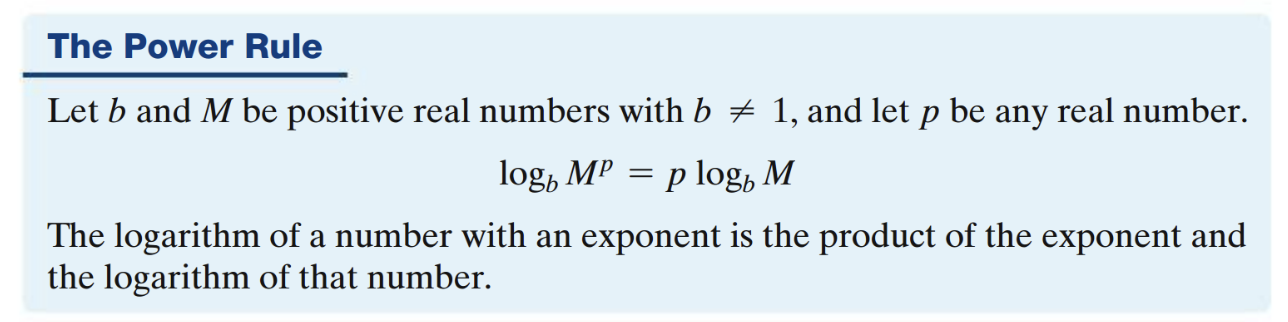
\includegraphics[scale=.7]{Chapter 6/6.6-figure3.png}}
Let's take a look at why this is true with an example:

\vspace{50mm}

\underline{\textbf{Example 3 - Using the Power Rule for Logarithms}}

Use the power rule to expand each of the logarithmic expressions:
\begin{multicols}{3}
    \begin{enumerate}[(a)]
    \item $\D \log_57^4$
    \item $\D \ln \sqrt{x}$
    \item $\D \log(4x)^5$
\end{enumerate}
\end{multicols}


\newpage

\textbf{{\large Expanding Logarithmic Expressions}}

As we have seen, in some situations we need to use more than one property of logarithms when expanding a logarithmic expression. In summary, these are the rules to expand logarithmic expressions.

\centerline{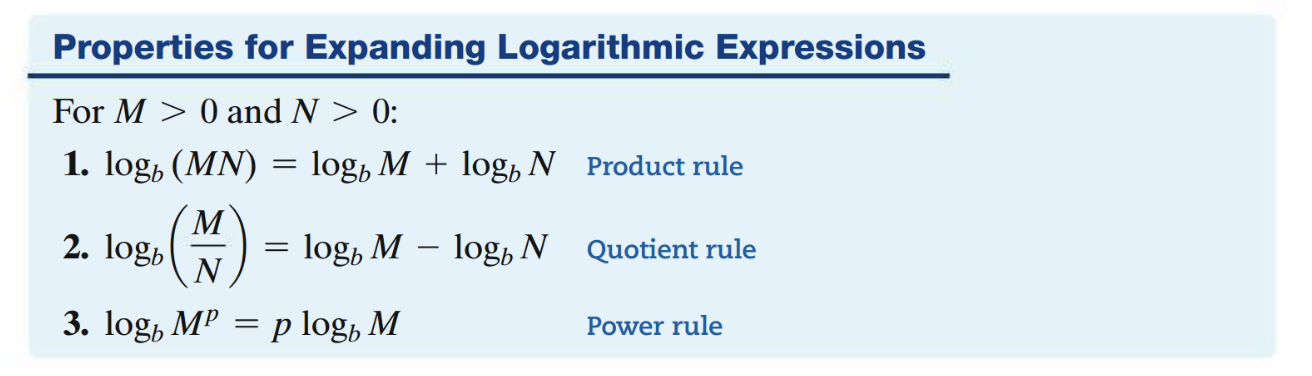
\includegraphics[scale=.6]{Chapter 6/6.6-figure4.png}}

\vspace{5mm}

Let's look at expanding some more complicated expressions. 

\underline{\textbf{Example 4 - Expanding Logarithmic Expressions}}

Use logarithmic properties to expand each expression as much as possible.
\begin{multicols}{2}
    \begin{enumerate}[(a)]
    \item $\D \log_b(x^2\sqrt{y})$
    \item $\D \log_6\left(\frac{\sqrt[3]{x}}{36y^4}\right)$
\end{enumerate}
\end{multicols}


\newpage
So far, we have been present with a single logarithmic expression or it was ``condensed" and then we expanded it. Now we go the other direction: given a logarithmic expression in expanded form, we want to condense it. 
\vspace{2mm}

\centerline{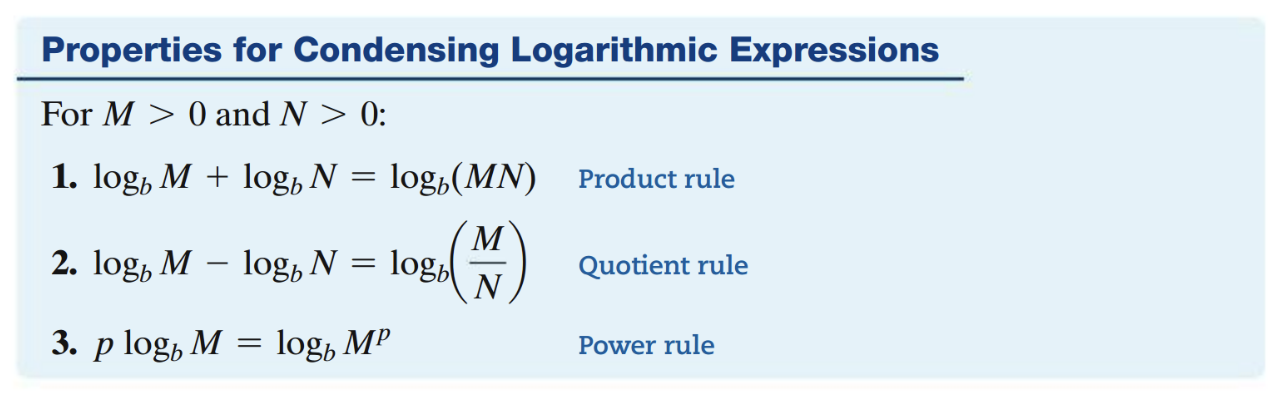
\includegraphics[scale=.6]{Chapter 6/6.6-figure5.png}}
\vspace{5mm}

\underline{\textbf{Example 5 - Condensing Logarithmic Expressions}}

Use logarithmic properties to write the following as a \textit{single} logarithm. 
\begin{multicols}{2}
    \begin{enumerate}[(a)]
    \item $\D \log_42 + \log_432$
    \item $\D \log (4x-3) - \log(x)$
\end{enumerate}
\end{multicols}

\newpage

\underline{\textbf{Example 6 - Condensing Logarithmic Expressions}}

Use logarithmic properties to write the following as a \textit{single} logarithm. 

    \begin{enumerate}[(a)]
    \item $\D \frac{1}{2}\log x + 4\log(x-1)$
    \vspace{50mm}
    \item $\D 3\ln(x+7)-\ln(x)$
    \vspace{50mm}
    \item $\D 3\log_b(x)-\log_b(6)-\frac{1}{2}\log_b(y)$
\end{enumerate}





\end{document}


